\documentclass[12pt]{extarticle}
\usepackage[francais]{babel}
\usepackage[utf8]{inputenc}
\usepackage[T1]{fontenc}
\usepackage{graphicx}
\usepackage{framed}
\usepackage[normalem]{ulem}
\usepackage{amsmath}
\usepackage{amsthm}
\usepackage{amssymb}
\usepackage{amsfonts}
\usepackage{enumerate}
\usepackage[top=1 in,bottom=1in, left=1 in, right=1 in]{geometry}
\usepackage{subcaption}
\usepackage[usenames,dvipsnames]{xcolor}

\title{Modèles épidémiologiques}
\date{30 janvier 2021}
\author{\textsc{BATY Léo}, \textsc{BRUNOD-INDRIGO Luca}}

\begin{document}

\maketitle

\section{Implémentation du modèle déterministe}

\subsection{Résolution du système différentiel}

Le modèle déterministe est implémenté dans le fichier \texttt{deterministic\_model}.
La méthode employée est un simple schéma d'Euler explicite qui calcule point par point une solution approchée des équations différentielles en remplaçant les dérivées par des différences finies sur un pas de temps $\delta t$ fixé.\\
Ainsi les équations utilisées s'écrivent : 

\begin{align*}
    s(t+\delta t) - s(t) &= -\beta i(t) s(t) \delta t\\
    i(t+\delta t) - i(t) &= (\beta s(t) - \gamma) i(t) \delta t\\
    r(t+\delta t) - r(t) &= \gamma i(t) \delta t
\end{align*}

\subsection{Calcul de limite théorique}

La limite théorique $r_\infty$ est calculée selon la formule vue en cours où $\mathcal{W}$ désigne la réciproque de la fonction de Lambert sur l'intervalle $]-1, +\infty[$: 

$$r_\infty = 1 + \frac{1}{R_0} \mathcal{W}(-R_0 e^{-R_0})$$

Pour le calcul de la fonction de Lambert réciproque dans le code, nous avons utilisé la librairie \texttt{Julia} consacrée : \texttt{LambertW}.

\subsection{Application numérique}

Le calcul théorique de $r_\infty$ étant valable pour le cas limite où $i(0) = 0^+$, il est nécessaire de choisir une valeur de $i(0)$ "petite" mais strictement positive (sans quoi la solution du système différentiel est trivialement constante à l'état initial).\\

\bigskip

La figure \ref{fig:deterministic} montre le tracé issu de la simulation du modèle déterministe pour les paramètres suivants : 
\begin{itemize}
    \item[-] $\beta = 0.1$
    \item[-] $\gamma = 0.05$
    \item[-] $i(0) = 0.001$ 
\end{itemize}

\begin{figure}[h!]
    \begin{center}
        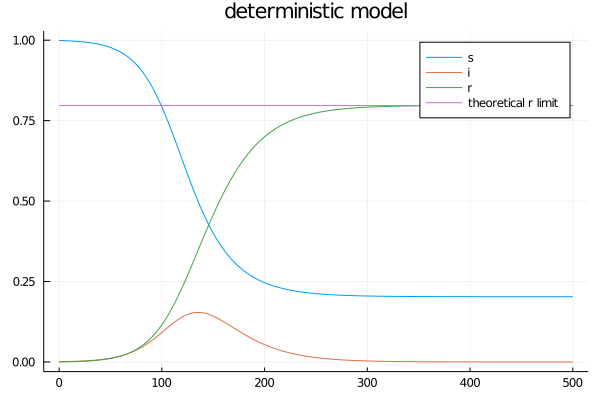
\includegraphics[width=0.5\linewidth]{figures/deterministic.png}
        \caption{Modèle déterministe et $r_\infty$ théorique}
        \label{fig:deterministic}
    \end{center}
\end{figure}

\bigskip

On constate que la limite théorique calculée semble bien correspondre à la valeur limite de la courbe $r$.
Notons que le choix de valeurs de $i(0)$ plus élevés qui éloignent du cas où la valeur est négligeable mènent à des écarts visibles entre les courbes $r$ et $r_\infty$, comme on peut s'y attendre.

\section{Implémentation du modèle Markovien}

\subsection{Description du modèle Markovien}

Le modèle Markovien est implémenté dans le fichier \texttt{markovian\_model.jl}.\\
Il correspond au modèle vu en cours avec une population de taille fixe $N$, un espace d'états 
$$E_N = \{(S, I, R) \in \mathbb{N}^3 \; S+I+R = N\}$$ 
et caractérisé par les transitions suivantes : 

\begin{itemize}
    \item[-] $(S, I, R) \rightarrow (S-1, I+1, R)$ au taux $\beta I \frac{S}{N}$
    \item[-] $(S, I, R) \rightarrow (S, I-1, R+1)$ au taux $\gamma I$
\end{itemize}

La figure \ref{fig:markovian} montre un exemple de simulation du processus de Markov avec les paramètres suivants : 
\begin{itemize}
    \item[-] $\beta = 0.1$
    \item[-] $\gamma = 0.05$
    \item[-] $N = 5000$ 
    \item[-] $X_0 = (S_0, I_0, R_0) = (4995, 5, 0)$ 
\end{itemize}

\begin{figure}[h!]
    \begin{center}
        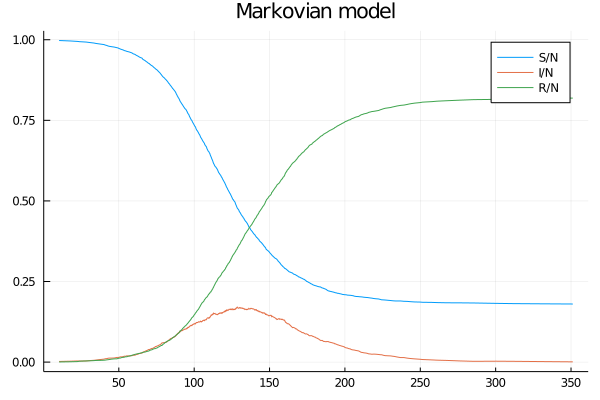
\includegraphics[width=0.5\linewidth]{figures/markovian.png}
        \caption{Processus de Markov renormalisé}
        \label{fig:markovian}
    \end{center}
\end{figure}

\subsection{Influence de $\beta$ et $\gamma$ sur l'état final}

Le choix des paramètres $\beta$ et $\gamma$ influence la forme des courbes issues de la simulation du processus de Markov et en particulier l'état final su système (lorsque le nombre d'individus infectés tombe à zéro et qu'il n'y a plus d'évolution).
La figure \ref{fig:final states} montre deux exemples de simulations avec une même taille de population $N = 100000$ et un même nombre d'individus infectés initialement $I_0 = 100$ mais avec des valeurs de $\beta$ différentes. 

\begin{figure}[h!]
    \begin{subfigure}{.5\textwidth}
        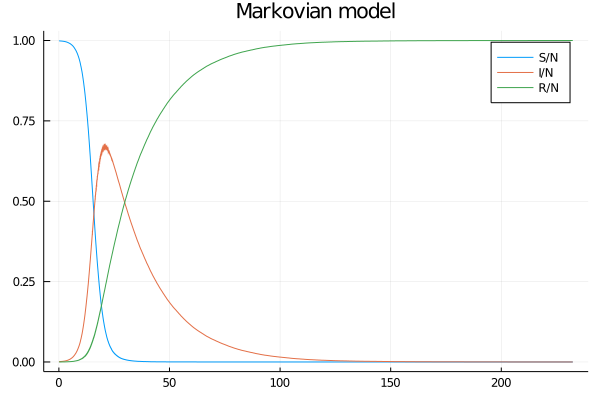
\includegraphics[width=0.8\linewidth]{figures/markovian_all_retired.png}
        \caption{$\beta = 0.5, \; \gamma = 0.05$}
    \end{subfigure}
    \begin{subfigure}{.5\textwidth}
        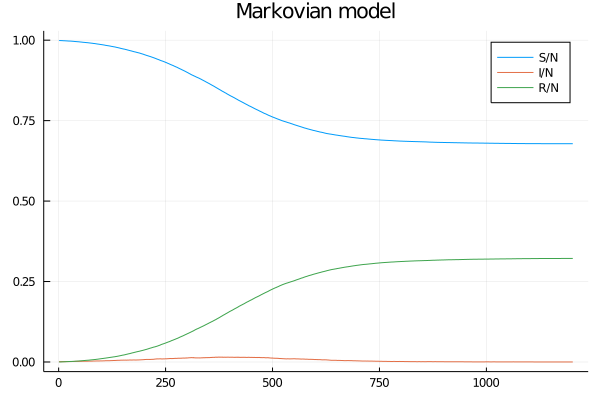
\includegraphics[width=0.8\linewidth]{figures/markovian_stable.png}
        \caption{$\beta = 0.06, \; \gamma = 0.05$}
    \end{subfigure}
    \caption{Simulations du processus de Markov pour différents paramètres}
    \label{fig:final states}
\end{figure}

Dans un cas, la valeur de $\beta$ élevée mène à une population entièrement retirée à l'état final tandis que dans l'autre cas une partie de la population reste susceptible.\\
Notons que les paramètres ont été choisis de sorte à avoir $R_0 > 1$ ce qui correspond à une limite théorique $r_\infty$ non nulle.

\section{Convergence du processus de Markov renormalisé}

La figure \ref{fig:convergence} montre les tracés issus du modèle déterministe et du modèle Markovien pour un même jeu de paramètres : 
\begin{itemize}
    \item[-] $\beta = 0.1$
    \item[-] $\gamma = 0.05$
\end{itemize}
et pour différentes valeurs de $N$ et de $I_0$ vérifiant : 
$$\frac{I_0}{N} = i(0) = 0.001$$

\begin{figure}[h!]
    \begin{subfigure}{.5\textwidth}
        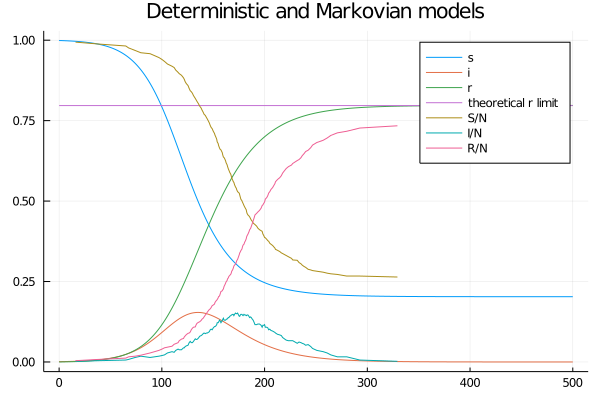
\includegraphics[width=0.8\linewidth]{figures/figureN_1000_initialI_1.png}
        \caption{$N = 1000, \; I_0 = 1$}
    \end{subfigure}
    \begin{subfigure}{.5\textwidth}
        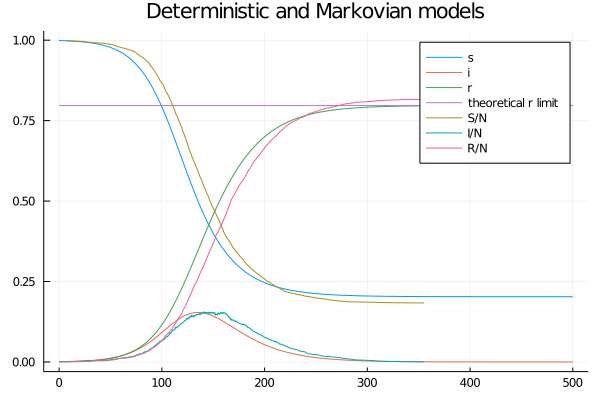
\includegraphics[width=0.8\linewidth]{figures/figureN_5000_initialI_5.png}
        \caption{$N = 5000, \; I_0 = 5$}
    \end{subfigure}
    \begin{subfigure}{.5\textwidth}
        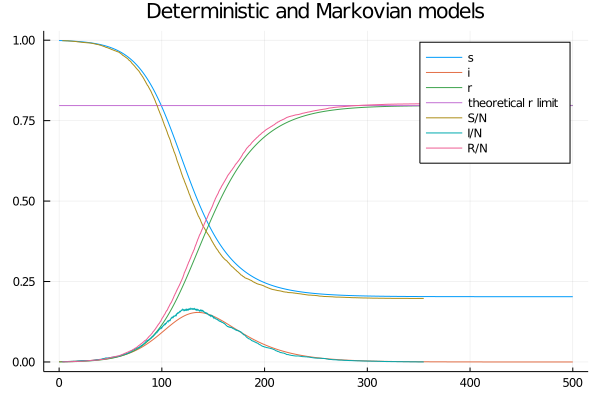
\includegraphics[width=0.8\linewidth]{figures/figureN_10000_initialI_10.png}
        \caption{$N = 10000, \; I_0 = 10$}
    \end{subfigure}
    \begin{subfigure}{.5\textwidth}
        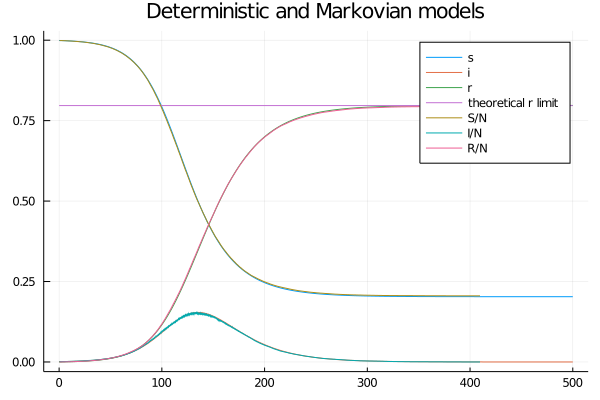
\includegraphics[width=0.8\linewidth]{figures/figureN_100000_initialI_100.png}
        \caption{$N = 100000, \; I_0 = 100$}
    \end{subfigure}
    \caption{Comparaison entre modèle déterministe et processus de Markov renormalisé}
    \label{fig:convergence}
\end{figure}

Nous pouvons constater que plus la taille de la population $N$ augmente, plus les courbes obtenues par simulation du processus de Markov sont proches des courbes issues du modèle déterministe partant de $i(0) = \frac{I_0}{N}$.\\
Les tracés, de même que les écarts entre les courbes restent bien entendu aléatoires et sont d'autant plus sensibles à l'aléa que $N$ est petit.
Ainsi, il a pu arriver lors de nos essais que des valeurs de $N$ relativement faibles donnent "par chance" des courbes presque confondues.
Pour l'illustration, nous avons conservé des simulations présentant des écarts qui nous ont semblé représentatifs.


\section{Question ouverte : estimation pratique de $\beta$ et $\gamma$}

Les équations différentielles du modèle SIR déterministe sont les suivantes : 
\begin{align*}
    \frac{ds}{dt}(t) &= -\beta i(t) s(t)\\
    \frac{di}{dt}(t) &= (\beta s(t) - \gamma) i(t)\\
    \frac{dr}{dt}(t) &= \gamma i(t)
\end{align*}

Un obstacle évident dans l'estimation de $\beta$ et $\gamma$ en partant des données hospitalières de Santé Publique France est que les fonctions $s(t)$, $i(t)$ et $r(t)$ ainsi que leurs dérivées sont inconues.
Nous proposons donc de nous placer dans les hypothèses suivantes qui nous semblent pertinentes et permettent de pallier le manque de données : 
\begin{enumerate}
    \item La proportion $h(t)$ de personnes hospitalisées est une fraction constante de la population infectée : $\exists \alpha \in [0, 1], \; h(t) = \alpha i(t) \; \forall t$
    \item De la même façon, la proportion $r_h(t)$ de personnes retirées après avoir été hospitalisées est une fraction de la population totale retirée avec le même facteur : $r_h(t) = \alpha r(t) \; \forall t$
    \item La proportion d'individus susceptibles est proche de 1 (début d'épidémie) : $s(t) \approx 1$
    \item Le paramètre $\gamma$ est identique pour la population hospitalisée et pour le reste de la population
    \item La proportion $h(t)$ de la population hospitalisée pour cause de Covid-19 est connue (il suffit de sommer les variations à partir d'un jour donné, mais ce chiffre ne figure pas dans les fichiers)
\end{enumerate}

\bigskip

Avec ces hypothèses, on peut écrire :
\begin{align*}
    \frac{di}{dt}(t) \approx (\beta - \gamma) i(t)  &\Leftrightarrow \alpha \frac{di}{dt}(t) \approx (\beta - \gamma) \alpha i(t)\\
                                                    &\Leftrightarrow \frac{dh}{dt}(t) \approx (\beta - \gamma) h(t)
\end{align*}
Ainsi que :
\begin{align*}
    \frac{dr}{dt}(t) = \gamma i(t)  &\Leftrightarrow \alpha \frac{dr}{dt}(t) = \gamma \alpha i(t)\\
                                                    &\Leftrightarrow \frac{dr_h}{dt}(t) = \gamma h(t)
\end{align*}

\bigskip

On a donc pour tout $t$ : 
\begin{align*}
    \beta &= \frac{1}{h(t)}(\frac{dh}{dt}(t) + \frac{dr_h}{dt}(t))\\
    \gamma &= \frac{1}{h(t)}\frac{dr_h}{dt}(t)
\end{align*}

On pourra donc calculer des estimations $\hat\beta$ et $\hat\gamma$ des paramètres en moyennant sur un certain nombre de jours, ce qui revient à minimiser la somme des écarts quadratiques : 
\begin{align*}
    \hat\beta &= \frac{1}{t_2 - t_1}\sum_{t = t_1}^{t_2}\frac{1}{h(t)}(\frac{dh}{dt}(t) + \frac{dr_h}{dt}(t))\\
    \hat\gamma &= \frac{1}{t_2 - t_1}\sum_{t = t_1}^{t_2}\frac{1}{h(t)}\frac{dr_h}{dt}(t)
\end{align*}

Pour l'application numérique des formules obtenues, les valeurs de $h(t)$ sont supposées connues et les dérivées $\frac{dh}{dt}$ et $\frac{dr_h}{dt}$ peuvent être approchées respectivement à partir des variations journalières du nombre de patients hospitalisés et du nombre de décès et de retours à domicile.


\end{document}
